\hypertarget{vn__math_8h}{}\section{src/hammerhead/hardware\+\_\+stack/vectornav/include/vectornav/vn\+\_\+math.h File Reference}
\label{vn__math_8h}\index{src/hammerhead/hardware\+\_\+stack/vectornav/include/vectornav/vn\+\_\+math.\+h@{src/hammerhead/hardware\+\_\+stack/vectornav/include/vectornav/vn\+\_\+math.\+h}}
{\ttfamily \#include \char`\"{}vn\+\_\+linear\+Algebra.\+h\char`\"{}}\\*
{\ttfamily \#include \char`\"{}vn\+\_\+kinematics.\+h\char`\"{}}\\*
Include dependency graph for vn\+\_\+math.\+h\+:
\nopagebreak
\begin{figure}[H]
\begin{center}
\leavevmode
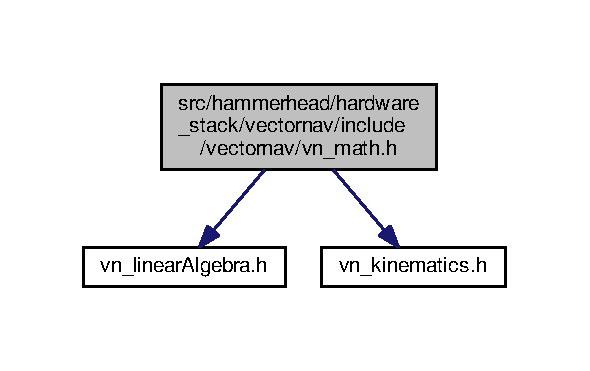
\includegraphics[width=283pt]{vn__math_8h__incl}
\end{center}
\end{figure}
This graph shows which files directly or indirectly include this file\+:
\nopagebreak
\begin{figure}[H]
\begin{center}
\leavevmode
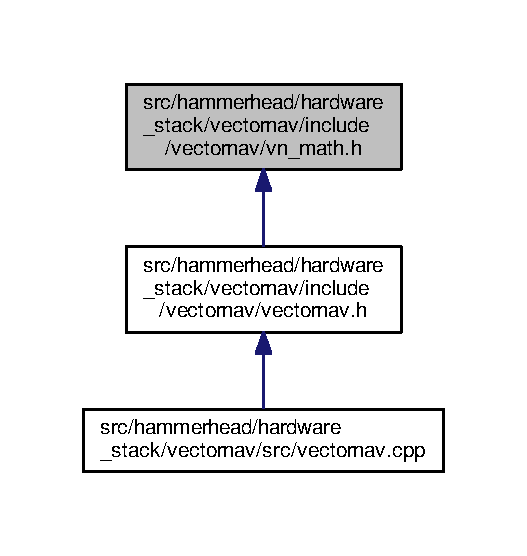
\includegraphics[width=253pt]{vn__math_8h__dep__incl}
\end{center}
\end{figure}


\subsection{Detailed Description}
\hypertarget{index_LICENSE}{}\subsection{L\+I\+C\+E\+N\+SE}\label{index_LICENSE}
M\+IT License (M\+IT)

Copyright (c) 2011 Vector\+Nav Technologies, L\+LC

Permission is hereby granted, free of charge, to any person obtaining a copy of this software and associated documentation files (the \char`\"{}\+Software\char`\"{}), to deal in the Software without restriction, including without limitation the rights to use, copy, modify, merge, publish, distribute, sublicense, and/or sell copies of the Software, and to permit persons to whom the Software is furnished to do so, subject to the following conditions\+:

The above copyright notice and this permission notice shall be included in all copies or substantial portions of the Software.

T\+HE S\+O\+F\+T\+W\+A\+RE IS P\+R\+O\+V\+I\+D\+ED \char`\"{}\+A\+S I\+S\char`\"{}, W\+I\+T\+H\+O\+UT W\+A\+R\+R\+A\+N\+TY OF A\+NY K\+I\+ND, E\+X\+P\+R\+E\+SS OR I\+M\+P\+L\+I\+ED, I\+N\+C\+L\+U\+D\+I\+NG B\+UT N\+OT L\+I\+M\+I\+T\+ED TO T\+HE W\+A\+R\+R\+A\+N\+T\+I\+ES OF M\+E\+R\+C\+H\+A\+N\+T\+A\+B\+I\+L\+I\+TY, F\+I\+T\+N\+E\+SS F\+OR A P\+A\+R\+T\+I\+C\+U\+L\+AR P\+U\+R\+P\+O\+SE A\+ND N\+O\+N\+I\+N\+F\+R\+I\+N\+G\+E\+M\+E\+NT. IN NO E\+V\+E\+NT S\+H\+A\+LL T\+HE A\+U\+T\+H\+O\+RS OR C\+O\+P\+Y\+R\+I\+G\+HT H\+O\+L\+D\+E\+RS BE L\+I\+A\+B\+LE F\+OR A\+NY C\+L\+A\+IM, D\+A\+M\+A\+G\+ES OR O\+T\+H\+ER L\+I\+A\+B\+I\+L\+I\+TY, W\+H\+E\+T\+H\+ER IN AN A\+C\+T\+I\+ON OF C\+O\+N\+T\+R\+A\+CT, T\+O\+RT OR O\+T\+H\+E\+R\+W\+I\+SE, A\+R\+I\+S\+I\+NG F\+R\+OM, O\+UT OF OR IN C\+O\+N\+N\+E\+C\+T\+I\+ON W\+I\+TH T\+HE S\+O\+F\+T\+W\+A\+RE OR T\+HE U\+SE OR O\+T\+H\+ER D\+E\+A\+L\+I\+N\+GS IN T\+HE S\+O\+F\+T\+W\+A\+RE.\hypertarget{vn__math_8h_DESCRIPTION}{}\subsection{D\+E\+S\+C\+R\+I\+P\+T\+I\+ON}\label{vn__math_8h_DESCRIPTION}
This header file provides access the math module of the Vector\+Nav C/\+C++ Library.

Notes
\begin{DoxyItemize}
\item Indexes used within the math library use 0 based indexing. For example, the first component of a 3 dimensional vector is referenced in code as vector3-\/$>$c0. 
\end{DoxyItemize}